\documentclass[class=minimal,border=0pt]{standalone}
\usepackage{bm}
\usepackage{amsmath}

\usepackage{tikz}
\usepackage{tikz-qtree}
\usetikzlibrary{trees} 
\usetikzlibrary{shapes.geometric}
\usetikzlibrary{mindmap,backgrounds}
\usetikzlibrary{positioning,shapes,shadows,arrows,calc}

\definecolor{lightgrey}{RGB}{214, 214, 210}
\definecolor{darkred}{RGB}{56,173,0}

\thispagestyle{empty}

\begin{document}
%\changefont{cmtt}{m}{n}

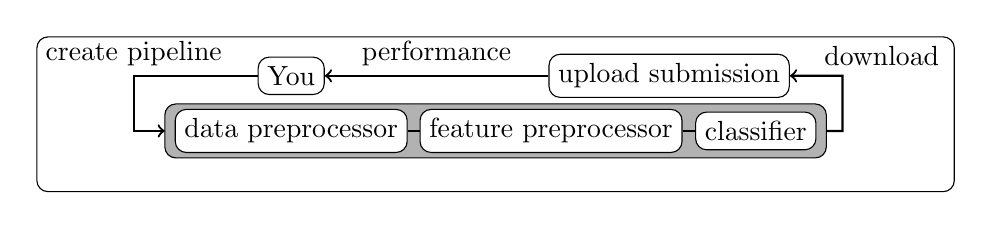
\begin{tikzpicture}[node distance=3cm, 
data/.style ={rectangle, text centered, fill=lightgrey},
activity/.style ={rectangle, draw=black, rounded corners, text centered, fill=white},
input/.style ={->,thick},
rinput/.style ={<-,thick},
output/.style ={->,thick},
connection/.style ={-,thick},
]


\node (DATAPRE) [activity, node distance=4.2cm] {data preprocessor};
\node (FEATPRE) [activity, right of=DATAPRE, node distance=3.3cm] {feature preprocessor};
\node (CLASS) [activity, right of=FEATPRE, node distance=2.6cm] {classifier};
\node (CODA) [activity, above of=FEATPRE, node distance=0.7cm, xshift=1.5cm] {upload submission};
\node (OPTI) [activity, above of=DATAPRE, node distance=0.7cm] {You};


\draw[connection] (DATAPRE) -- (FEATPRE);
\draw[connection] (FEATPRE) -- (CLASS);

\draw[input] (OPTI.west) -| node[above] {create pipeline} (-2,0.7) -- (-2, 0) -- ($(DATAPRE.west)-(0.125,0)$);
\draw[output] ($(CLASS.east)-(-0.125,0)$) -- (7,0) -- (7, 0.7) node[above, xshift=0.5cm] {download} -- ($(CODA.east)$);
\draw[input] (CODA) -- node[above] {performance} (OPTI);
%\draw[rinput] (OPTI.east) -- (9,0.7) -| ($(CLASS.north)-(0,-0.125)$);

\begin{pgfonlayer}{background}
  % Configuration Process, better don't touch
  \path (OPTI.north -| DATAPRE.west)+(-1.75,0.25) node (resUL) {};
  \path (CLASS.east |- CLASS.south)+(1.75,-0.525) node(resBR) {};
  \path [rounded corners, draw=black, fill=white] (resUL) rectangle (resBR);
  \path (CLASS.west |- CLASS.south) node [align=left, anchor=west, text=black] {};
\end{pgfonlayer}

\begin{pgfonlayer}{background}
  % pipeline Process, better don't touch
  \path (DATAPRE.north -| DATAPRE.west)+(-0.125,0.0625) node (resUL) {};
  \path (CLASS.east |- FEATPRE.south)+(0.125,-0.0625) node(resBR) {};
  \path [rounded corners, draw=black, fill=black!30] (resUL) rectangle (resBR);
\end{pgfonlayer}




\end{tikzpicture}


\end{document}
